% Options for packages loaded elsewhere
\PassOptionsToPackage{unicode}{hyperref}
\PassOptionsToPackage{hyphens}{url}
\PassOptionsToPackage{dvipsnames,svgnames,x11names}{xcolor}
%
\documentclass[
  oneside,
  open=any]{scrreprt}

\usepackage{amsmath,amssymb}
\usepackage{iftex}
\ifPDFTeX
  \usepackage[T1]{fontenc}
  \usepackage[utf8]{inputenc}
  \usepackage{textcomp} % provide euro and other symbols
\else % if luatex or xetex
  \usepackage{unicode-math}
  \defaultfontfeatures{Scale=MatchLowercase}
  \defaultfontfeatures[\rmfamily]{Ligatures=TeX,Scale=1}
\fi
\usepackage{lmodern}
\ifPDFTeX\else  
    % xetex/luatex font selection
\fi
% Use upquote if available, for straight quotes in verbatim environments
\IfFileExists{upquote.sty}{\usepackage{upquote}}{}
\IfFileExists{microtype.sty}{% use microtype if available
  \usepackage[]{microtype}
  \UseMicrotypeSet[protrusion]{basicmath} % disable protrusion for tt fonts
}{}
\makeatletter
\@ifundefined{KOMAClassName}{% if non-KOMA class
  \IfFileExists{parskip.sty}{%
    \usepackage{parskip}
  }{% else
    \setlength{\parindent}{0pt}
    \setlength{\parskip}{6pt plus 2pt minus 1pt}}
}{% if KOMA class
  \KOMAoptions{parskip=half}}
\makeatother
\usepackage{xcolor}
\usepackage[showframe,inner=2cm,outer=2cm,top=3cm,bottom=4cm,headsep=22pt,headheight=11pt,footskip=33pt,ignorehead,ignorefoot,heightrounded]{geometry}
\setlength{\emergencystretch}{3em} % prevent overfull lines
\setcounter{secnumdepth}{5}
% Make \paragraph and \subparagraph free-standing
\makeatletter
\ifx\paragraph\undefined\else
  \let\oldparagraph\paragraph
  \renewcommand{\paragraph}{
    \@ifstar
      \xxxParagraphStar
      \xxxParagraphNoStar
  }
  \newcommand{\xxxParagraphStar}[1]{\oldparagraph*{#1}\mbox{}}
  \newcommand{\xxxParagraphNoStar}[1]{\oldparagraph{#1}\mbox{}}
\fi
\ifx\subparagraph\undefined\else
  \let\oldsubparagraph\subparagraph
  \renewcommand{\subparagraph}{
    \@ifstar
      \xxxSubParagraphStar
      \xxxSubParagraphNoStar
  }
  \newcommand{\xxxSubParagraphStar}[1]{\oldsubparagraph*{#1}\mbox{}}
  \newcommand{\xxxSubParagraphNoStar}[1]{\oldsubparagraph{#1}\mbox{}}
\fi
\makeatother

\providecommand{\tightlist}{%
  \setlength{\itemsep}{0pt}\setlength{\parskip}{0pt}}\usepackage{longtable,booktabs,array}
\usepackage{calc} % for calculating minipage widths
% Correct order of tables after \paragraph or \subparagraph
\usepackage{etoolbox}
\makeatletter
\patchcmd\longtable{\par}{\if@noskipsec\mbox{}\fi\par}{}{}
\makeatother
% Allow footnotes in longtable head/foot
\IfFileExists{footnotehyper.sty}{\usepackage{footnotehyper}}{\usepackage{footnote}}
\makesavenoteenv{longtable}
\usepackage{graphicx}
\makeatletter
\def\maxwidth{\ifdim\Gin@nat@width>\linewidth\linewidth\else\Gin@nat@width\fi}
\def\maxheight{\ifdim\Gin@nat@height>\textheight\textheight\else\Gin@nat@height\fi}
\makeatother
% Scale images if necessary, so that they will not overflow the page
% margins by default, and it is still possible to overwrite the defaults
% using explicit options in \includegraphics[width, height, ...]{}
\setkeys{Gin}{width=\maxwidth,height=\maxheight,keepaspectratio}
% Set default figure placement to htbp
\makeatletter
\def\fps@figure{htbp}
\makeatother
% definitions for citeproc citations
\NewDocumentCommand\citeproctext{}{}
\NewDocumentCommand\citeproc{mm}{%
  \begingroup\def\citeproctext{#2}\cite{#1}\endgroup}
\makeatletter
 % allow citations to break across lines
 \let\@cite@ofmt\@firstofone
 % avoid brackets around text for \cite:
 \def\@biblabel#1{}
 \def\@cite#1#2{{#1\if@tempswa , #2\fi}}
\makeatother
\newlength{\cslhangindent}
\setlength{\cslhangindent}{1.5em}
\newlength{\csllabelwidth}
\setlength{\csllabelwidth}{3em}
\newenvironment{CSLReferences}[2] % #1 hanging-indent, #2 entry-spacing
 {\begin{list}{}{%
  \setlength{\itemindent}{0pt}
  \setlength{\leftmargin}{0pt}
  \setlength{\parsep}{0pt}
  % turn on hanging indent if param 1 is 1
  \ifodd #1
   \setlength{\leftmargin}{\cslhangindent}
   \setlength{\itemindent}{-1\cslhangindent}
  \fi
  % set entry spacing
  \setlength{\itemsep}{#2\baselineskip}}}
 {\end{list}}
\usepackage{calc}
\newcommand{\CSLBlock}[1]{\hfill\break\parbox[t]{\linewidth}{\strut\ignorespaces#1\strut}}
\newcommand{\CSLLeftMargin}[1]{\parbox[t]{\csllabelwidth}{\strut#1\strut}}
\newcommand{\CSLRightInline}[1]{\parbox[t]{\linewidth - \csllabelwidth}{\strut#1\strut}}
\newcommand{\CSLIndent}[1]{\hspace{\cslhangindent}#1}


\usepackage{booktabs}
\usepackage{longtable}
\usepackage{array}
\usepackage{multirow}
\usepackage{wrapfig}
\usepackage{float}
\usepackage{colortbl}
\usepackage{pdflscape}
\usepackage{tabu}
\usepackage{threeparttable}
\usepackage{threeparttablex}
\usepackage[normalem]{ulem}
\usepackage{makecell}
\usepackage{xcolor}
\usepackage{xcolor}
\usepackage{lipsum}
\usepackage{glossaries}
\usepackage{booktabs}
\usepackage{hyperref}
\usepackage[capitalise,noabbrev]{cleveref}
\makeatletter
\@ifpackageloaded{caption}{}{\usepackage{caption}}
\AtBeginDocument{%
\ifdefined\contentsname
  \renewcommand*\contentsname{Table des matières}
\else
  \newcommand\contentsname{Table des matières}
\fi
\ifdefined\listfigurename
  \renewcommand*\listfigurename{Liste des Figures}
\else
  \newcommand\listfigurename{Liste des Figures}
\fi
\ifdefined\listtablename
  \renewcommand*\listtablename{Liste des Tables}
\else
  \newcommand\listtablename{Liste des Tables}
\fi
\ifdefined\figurename
  \renewcommand*\figurename{Figure}
\else
  \newcommand\figurename{Figure}
\fi
\ifdefined\tablename
  \renewcommand*\tablename{Table}
\else
  \newcommand\tablename{Table}
\fi
}
\@ifpackageloaded{float}{}{\usepackage{float}}
\floatstyle{ruled}
\@ifundefined{c@chapter}{\newfloat{codelisting}{h}{lop}}{\newfloat{codelisting}{h}{lop}[chapter]}
\floatname{codelisting}{Listing}
\newcommand*\listoflistings{\listof{codelisting}{Liste des Listings}}
\makeatother
\makeatletter
\makeatother
\makeatletter
\@ifpackageloaded{caption}{}{\usepackage{caption}}
\@ifpackageloaded{subcaption}{}{\usepackage{subcaption}}
\makeatother

\usepackage{hyphenat}
\usepackage{ifthen}
\usepackage{calc}
\usepackage{calculator}



\usepackage{graphicx}
\usepackage{geometry}
\usepackage{afterpage}
\usepackage{tikz}
\usetikzlibrary{calc}
\usetikzlibrary{fadings}
\usepackage[pagecolor=none]{pagecolor}


% Set the titlepage font families







% Set the coverpage font families


\ifLuaTeX
\usepackage[bidi=basic]{babel}
\else
\usepackage[bidi=default]{babel}
\fi
\babelprovide[main,import]{french}
% get rid of language-specific shorthands (see #6817):
\let\LanguageShortHands\languageshorthands
\def\languageshorthands#1{}
\ifLuaTeX
  \usepackage{selnolig}  % disable illegal ligatures
\fi
\usepackage{bookmark}

\IfFileExists{xurl.sty}{\usepackage{xurl}}{} % add URL line breaks if available
\urlstyle{same} % disable monospaced font for URLs
\hypersetup{
  pdftitle={Classification de toute allure!},
  pdflang={fr},
  colorlinks=true,
  linkcolor={blue},
  filecolor={Maroon},
  citecolor={Blue},
  urlcolor={Blue},
  pdfcreator={LaTeX via pandoc}}


\title{Classification de toute allure!}
\usepackage{etoolbox}
\makeatletter
\providecommand{\subtitle}[1]{% add subtitle to \maketitle
  \apptocmd{\@title}{\par {\large #1 \par}}{}{}
}
\makeatother
\subtitle{Une analyse de la relation entre l'étiquette et le cheminement
de circuits dans Trackmania Nations Forever utilisant la classification}
\author{Nicolas Kmita}
\date{}

\begin{document}
%%%%% begin titlepage extension code


\begin{titlepage}

%%% TITLE PAGE START

% Set up alignment commands
%Page
\newcommand{\titlepagepagealign}{
\ifthenelse{\equal{center}{right}}{\raggedleft}{}
\ifthenelse{\equal{center}{center}}{\centering}{}
\ifthenelse{\equal{center}{left}}{\raggedright}{}
}


\newcommand{\titleandsubtitle}{
% Title and subtitle
{\fontsize{30}{36.0}\selectfont
{\uppercase{\nohyphens{Classification de toute allure!}}}\par
}%

\vspace{\betweentitlesubtitle}
{
{\Large{\textit{\nohyphens{Une analyse de la relation entre l'étiquette
et le cheminement de circuits dans Trackmania Nations Forever utilisant
la classification}}}}\par
}}
\newcommand{\titlepagetitleblock}{
\rule{\textwidth}{0.4pt} % Thin horizontal rule
\vspace{0.025\textheight} % Whitespace between the top rules and title

\titleandsubtitle

\vspace{0.025\textheight} 
\rule{0.3\textwidth}{0.4pt} % Short horizontal rule under the title
}
\newcommand{\authorstyle}[1]{{\Large{#1}}}

\newcommand{\affiliationstyle}[1]{{\large{#1}}}

\newcommand{\titlepageauthorblock}{
{\authorstyle{\nohyphens{Nicolas Kmita}\\}}
}

\newcommand{\titlepageaffiliationblock}{
\hangindent=1em
\hangafter=1
{\affiliationstyle{
{1}.~École secondaire Franco-Cité


\vspace{1\baselineskip} 
}}
}
\newcommand{\headerstyled}{%
{}
}
\newcommand{\footerstyled}{%
{\large{\textsc{M. Chabot\\
MDM4U\\
25 octobre 2024\\}}}
}
\newcommand{\datestyled}{%
{}
}


\newcommand{\titlepageheaderblock}{\headerstyled}

\newcommand{\titlepagefooterblock}{
\footerstyled
}

\newcommand{\titlepagedateblock}{
\datestyled
}

%set up blocks so user can specify order
\newcommand{\titleblock}{\newlength{\betweentitlesubtitle}
\setlength{\betweentitlesubtitle}{\baselineskip}
{

{\titlepagetitleblock}
}

\vspace{0.1\textheight}
}

\newcommand{\authorblock}{}

\newcommand{\affiliationblock}{}

\newcommand{\logoblock}{{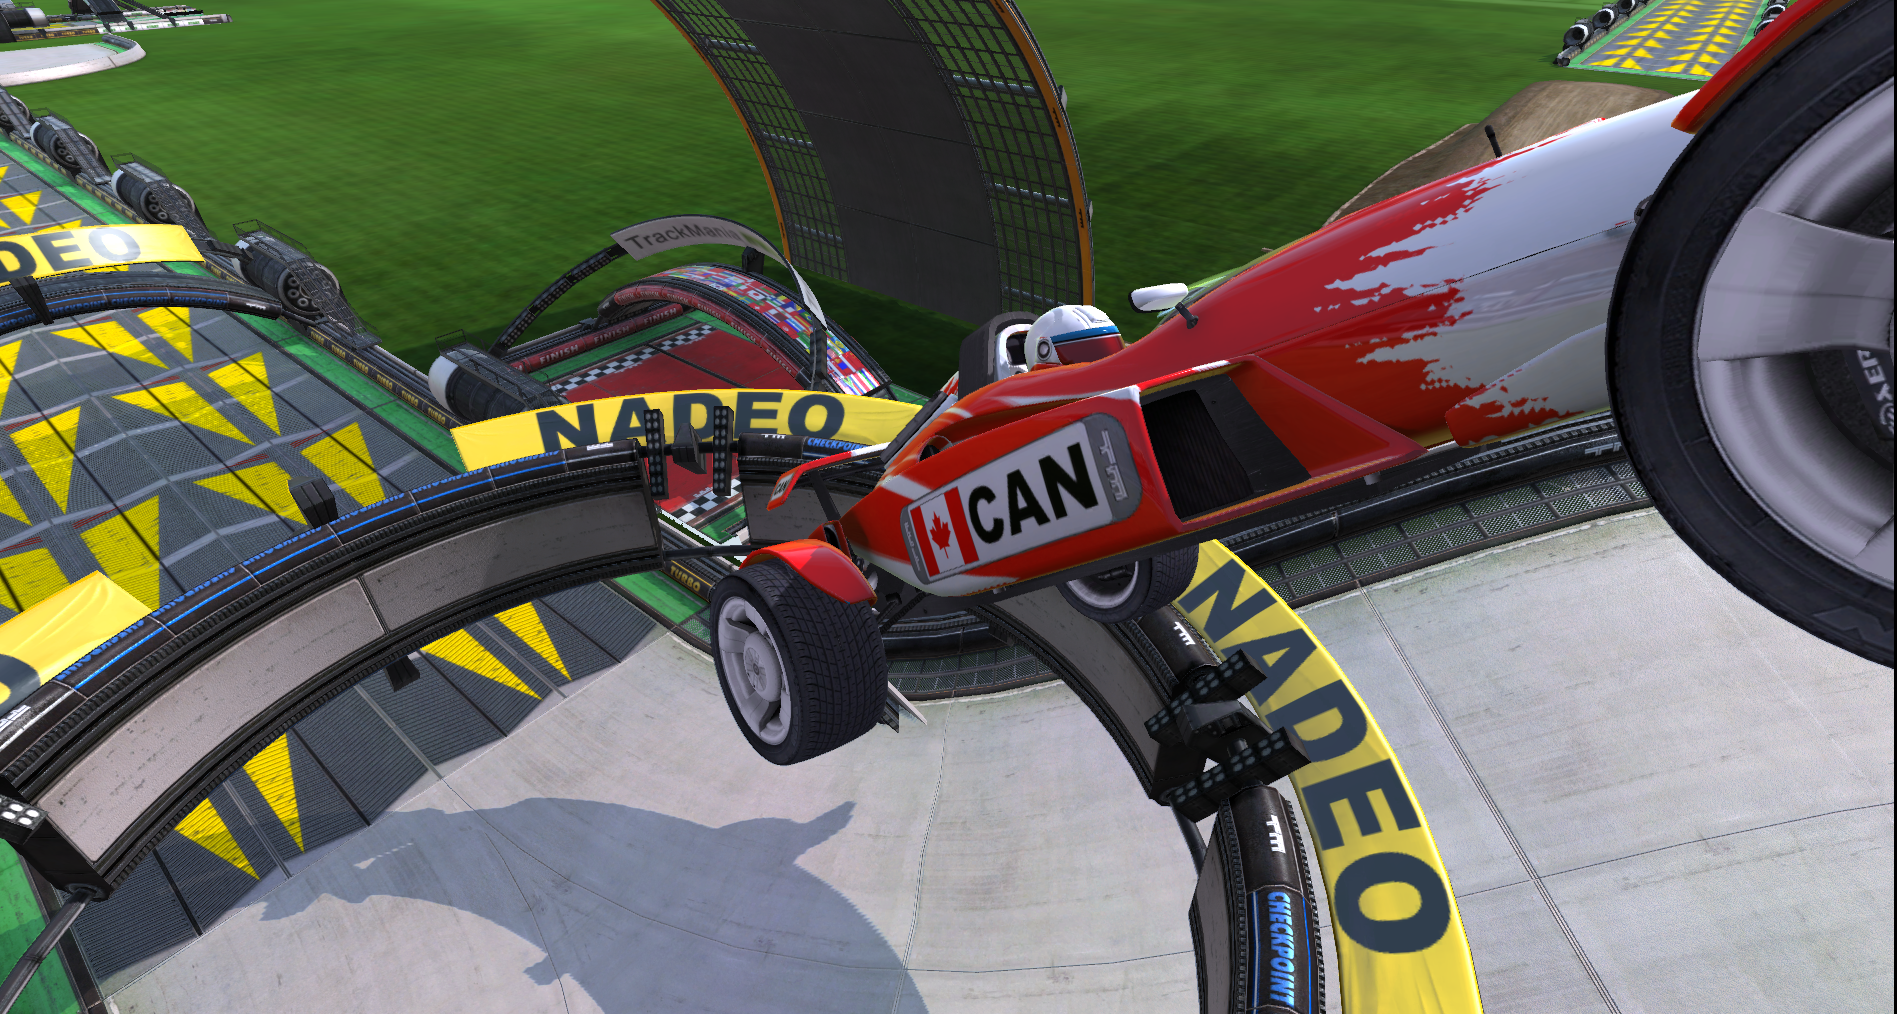
\includegraphics[width=0.7\textheight]{img/car-jump.png}}

\vspace{1cm}
}

\newcommand{\footerblock}{{\titlepagefooterblock}

\vspace{0pt}
}

\newcommand{\dateblock}{}

\newcommand{\headerblock}{}

\thispagestyle{empty} % no page numbers on titlepages


\newlength{\minipagewidth}
\setlength{\minipagewidth}{\textwidth}
\raggedright % single minipage
% [position of box][box height][inner position]{width}
% [s] means stretch out vertically; assuming there is a vfill
\begin{minipage}[b][\textheight][s]{\minipagewidth}
\titlepagepagealign
\titleblock

\authorblock

\logoblock

\footerblock
\par

\end{minipage}\ifthenelse{\equal{}{right} \OR \equal{}{leftright} }{
\hspace{\B}
\vrulecode}{}
\clearpage
%%% TITLE PAGE END
\end{titlepage}
\setcounter{page}{1}

%%%%% end titlepage extension code

\renewcommand*\contentsname{Table des matières}
{
\hypersetup{linkcolor=}
\setcounter{tocdepth}{2}
\tableofcontents
}

\begin{verbatim}
\end{verbatim}

\chapter{Glossaire}\label{glossaire}

\textbf{API}\quad{} Une API, soit une interface de programmation
d'applications, est l'interface entre un programme et un autre. Dans le
cas de cet article, l'API de TMNF-X est l'interface utilisée pour
communiquer avec la base de données de TMNF-X.

\quad

\textbf{Étiquette}\quad{} L'étiquette, ou « tag » en anglais, est le
descripteur principal d'un circuit. Il n'y a pas de définitions
officielles des différentes étiquettes de Trackmania Nations Forever,
toutefois, l'installation Trackmania 2020 a été fournie quelques
définitions des mêmes étiquettes. Les définitions fournies pour
Trackmania 2020 ne sont pas compatibles avec TMNF en raison des
différences majeures entre les deux installations.

Le nom étiquette peut mener à confusion en discutant de modèles de
classification puisqu'il y a la classification à classes multiples et à
étiquettes multiples. Les deux catégories de modèles sont entièrement
différentes. Le modèle d'amplification de gradients que nous utilisons
plus tard dans ce rapport utilise des classes multiples. Ainsi,
l'utilisation du terme « étiquette » en discutant du modèle fait
référence aux étiquettes de Trackmania et non des étiquettes par rapport
aux statistiques.

\quad

\textbf{TMNF}\quad{} TMNF est l'abréviation du titre Trackmania Nations
Forever, le jeu de course d'arcade analysé dans cet article.

\quad

\textbf{TMNF-X}\quad{} Le site Internet a pour but de partager, entre
joueurs, les créations reliées à Trackmania Nations Forever.

\quad

\textbf{Trackmania 2020}\quad{} L'installation du jeu Trackmania publié
en 2020.

\quad

\textbf{Rediffusion}\quad{} Une rediffusion du chemin que parcourt un
joueur. Aussi appelée « replay ».

\chapter{Introduction}\label{sec-intro}

Trackmania Nations Forever est la neuvième installation dans la série de
jeux vidéo Trackmania. Ce jeu de course d'arcade, sortie en 2008, n'a
que quatre entrées possibles: avancer, reculer, tourner vers la gauche,
et tourner vers la droite. C'est ainsi un jeu très abordable pour des
débutants. Il y a pourtant diverses fonctionnalités internes qui lui
donnent un plafond de compétences très élevé.

L'analyse statistique est très courante dans la série Trackmania afin de
s'améliorer au jeu, pour pousser les limites du possible, ou simplement
pour explorer une curiosité. Des joueurs, tels que JstAnothrVirtuoso
(JstAnothrVirtuoso 2024) et Yosh ({«~Yosh~»}, s.~d.), et des projets
comme Linesight (pb4git, et al 2024) sont de bons exemples. Ces deux
derniers ont même agi comme sources d'inspiration pour le thème général
de ce projet. Il y a également des outils tels que TMDojo (TeamDojo,
s.~d.) pour l'installation Trackmania de 2020 qui servent à donner de la
rétroaction rapide aux joueurs sur des circuits variés.

Les joueurs peuvent créer leurs propres circuits, ainsi que de les
publier sur des plateformes telles que Trackmania Nations Forever
Exchange, abrégé à TMNF-X. Les auteurs catégorisent leur circuit selon
le style et but, soit sous une étiquette. Il est à noter que les
étiquettes n'ont pas de définitions exactes, et que plus d'une étiquette
peut être assignée par circuit. Des étiquettes pourraient être «
Fullspeed », « LOL » ou un certain nombre d'autres qui sont indiquées
dans la Section~\ref{sec-method}.

Les étiquettes sont donc choisies selon l'opinion subjective de l'auteur
des étiquettes les plus appropriées. Les auteurs utilisent leur
interprétation des différences entre les caractéristiques de chaque
étiquette de circuit. Il est ainsi à se demander quelles
caractéristiques principales du cheminement de la voiture influencent
l'étiquette du circuit. Cette étude explora les relations entre le
cheminement de la voiture et l'étiquette du circuit.

\section{Définir un joueur compétent}\label{sec-competent}

Il faut d'abord définir les joueurs compétents, ceux auxquels les
rediffusions seront tirées.

Un joueur compétent devra être assez pratiqué à Trackmania Nations
Forever afin de bien représenter un circuit donné. Un joueur non
compétent, au contraire, ne pourra pas effectivement compléter un
circuit sans faire des actions aberrantes, telles qu'entrer en collision
avec des murs ou ralentir la voiture. Ce contraste permet de définir un
joueur compétent par négation: c'est un joueur qui ne fait peu
d'erreurs.

Notez que cette définition est subjective et ne représente pas tous les
joueurs compétents. C'est une définition à but d'augmenter la
représentativité du circuit par le cheminement de la voiture du joueur
considéré compétent.

La sélection de rediffusions de joueurs compétents est embrouillée par
le manque d'informations contextuelles ; le rang du joueur, son temps
total dans le jeu, et autres tels critères ne sont pas facilement
découvrables en cherchant un circuit donné et, plus important encore,
ces critères identifieraient les joueurs. Il est donc à faire recours à
des critères présentés pour chaque fichier de rediffusion.

Nous avons choisi de filtrer selon le nombre de joueurs ayant soumis une
rediffusion pour un circuit donné sur TMNF-X. Ce critère est (assez)
simple à filtrer au travers de l'API de TMNF-X et permet aux
rediffusions de rapprocher le cheminement le plus représentatif du
circuit. Le plus de rediffusions soumises, le plus haut le niveau de
compétition et, donc, le plus représentatif la rediffusion. Afin de bien
équilibrer une sélection représentative des circuits\footnote{Une
  filtration trop restrictive limitera les circuits sélectionnés à ceux
  qui sont très fameux, ayant des milliers de rediffusions soumis,
  plutôt que ceux qui ont une ou deux bonnes rediffusions.} et la
qualité des rediffusions\footnote{Les circuits ayant des milliers de
  rediffusions tendent, de notre expérience, à avoir des rediffusions
  poussées aux limites du possible.}, un joueur compétent sera défini,
dans cet article, en tant qu'un joueur tenant le record sur un circuit
donné, où ce circuit comporte au minimum cinq records soumis. En
choisissant cinq comme nombre minimal de rediffusions, nous espérons
minimiser le nombre de records insuffisamment représentatifs d'un
circuit par des joueurs ayant moins d'expérience.

Il est à noter qu'il se pourrait, toutefois, que plus de cinq joueurs
débutants décident, par chance ou par exprès, de soumettre leurs records
sur le même circuit.

\section{Questions}\label{questions}

Cette section couvre les questions provoquant l'étude actuelle.

\subsection{Exploration pré-modèle}\label{exploration-pruxe9-moduxe8le}

Il est fort probable que certaines techniques soient discernables avec
les variations de variables récoltées. Une telle technique pourrait être
la « grass-slide », où la voiture est positionnée à 90° et fait un
virage agressif (Tunachopps 2023). Dans ce cas, nous estimons une hausse
de vitesse angulaire et de vitesse latérale comparée au restant du
circuit. D'autres techniques/bogues potentiellement discernables
seraient la « edge-bogue », la « uber-bogue » et la « nose-bogue » qui
changent drastiquement le vecteur vitesse\footnote{Pour une
  démonstration, voir la vidéo par Kimura et al.}. Un aperçu de la
distribution de bogues ou autres provoquant de grands changements sera
visible par des graphiques à violons multiples de la différence maximale
et moyenne de vecteur vitesse selon l'étiquette et de la différence
maximale et moyenne de vitesse latérale selon l'étiquette. Sachant que
la définition de l'étiquette « PressForward » dans Trackmania 2020
indique la présence d'acrobaties normalement impossibles manuellement,
il est probable que de tels changements drastiques de vitesse soient
présents.

\section{Quel modèle de classification servira le mieux
?}\label{sec-which-model-hypothesis}

Plusieurs méthodes de classification de points de données existent,
ayant tous leurs cas d'utilisation, avantages et désavantages
différents. Pour le cas de la classification du cheminement dans une
étiquette, il y a cinq exigences principales.

Le modèle doit d'abord \textbf{classifier de manière tabulaire} afin de
pouvoir utiliser les données récoltées (« What is Tabular
Classification? »). De tels modèles sont les Transformeurs tabulaires et
k-NN (Keita, Zoumana 2024), etc.

Afin de réduire la complexité de l'analyse et de mener à un meilleur
contraste entre les étiquettes, le modèle devra
\textbf{prédire une étiquette}. Le modèle devrait pouvoir faire de la
classification à classe multiple afin de gérer le nombre d'étiquettes
possibles plus grand que deux\footnote{Soit une variable nominale non
  binaire.} (Keita, Zoumana 2024). En raison de la nécessité d'une
exclusivité mutuelle entre les classes (Keita, Zoumana 2024) pour la
classification à classes multiples, les circuits sélectionnés devront
être filtrés afin de ne garder que les circuits ayant une seule
étiquette assignée. De tels algorithmes, lorsque mis en série, sont la
forêt aléatoire, Bayes naïf, k-NN et amplification de gradients. Il est
à noter que la classification à étiquette multiple, telle que
l'amplification de gradients multiétiquettes (Keita, Zoumana 2024),
serait préférable afin de prédire et gérer plusieurs étiquettes
simultanément. Toutefois, ceci mènerait à une complexité hors de la
portée de ce projet.

Le modèle serait préférablement un \textbf{apprenant avide} afin de
présenter des tendances dans les données plutôt que de simplement
prédire selon les points de données les plus proches (Keita, Zoumana
2024). Une majorité des modèles respectent cette exigence, notamment à
l'exception du modèle k-NN qui est relativement simple comparé aux
autres modèles, mais qui cherche le voisin le plus près.

Le modèle devrait préférablement être \textbf{explicable}, soit par
l'utilisation d'une IAX\footnote{Intelligence artificielle explicable}
(Keita, Zoumana 2024). Puisque l'étude actuelle vise non seulement à
prédire l'étiquette, mais également à comprendre ce qui influe un choix
d'étiquette, il est préférable qu'une interprétabilité soit facilitée
pour le modèle choisi\footnote{Notez également que l'Europe a des
  réglementations, telles que le Règlement général sur la protection des
  données (Keita, Zoumana 2024), qui mandatent l'explication de
  décisions automatisées.}. Les IAXs sont habituellement des outils
post-prédiction servant à expliquer le raisonnement d'un modèle, donc
elles peuvent fonctionner avec une majorité des modèles existants. Des
exemples de techniques IAX sont SHAP (Awan, Abid Ali 2015), LIME et
l'explication contrefactuelle (Keita, Zoumana 2024).

Combinant toutes ces exigences, peu de modèles restent\footnote{De la
  liste des modèles trouvés lors de recherches.}. La combinaison de
techniques et de modèles qui, sans analyser les données profondément
d'avance, est prévue être la plus exacte et précise suit. Soit un modèle
d'arbre de décisions à classes multiples (Kattack, et al 2006), soit
d'amplification de gradient à classes multiple (Keita, Zoumana 2024),
servira probablement\footnote{La profondeur des subtilités de chaque
  méthode diminue la certitude de la méthode la plus représentative.} le
mieux pour classifier les nombreuses étiquettes. Si la méthode choisie
n'incorpore pas une explicabilité, telle que dans le cas de
l'amplification de gradient sans modifications (XGBoost 2022), la
technique IAX SHAP (Awan, Abid Ali 2015) est prédite de permettre la
meilleure explication des choix prise par le modèle.

Afin de déterminer le modèle le plus représentatif, les modèles peuvent
être comparés entre eux par moyen de leur précision, exactitude,
sensibilité, spécificité, score F1, ou courbe ROC\footnote{Certains
  indicateurs dépendent de distributions particulières des valeurs
  prédites. Par exemple, la spécificité est préférée lorsqu'il y a plus
  de faux positifs que de faux négatifs.} (Keita, Zoumana 2024).

Un modèle de simulacre sera d'abord utilisé afin d'assigner un point de
départ. Un modèle de régression logistique sera, ensuite, utilisé comme
modèle simple et souvent efficace. Finalement, un modèle d'amplification
de gradients est prévu être le plus représentatif.

\section{Que peut être déduit au sujet des affectants de l'étiquette
résultante grâce aux modèles
?}\label{que-peut-uxeatre-duxe9duit-au-sujet-des-affectants-de-luxe9tiquette-ruxe9sultante-gruxe2ce-aux-moduxe8les}

Utilisant les définitions fournies pour Trackmania 2020 comme base, nous
croyons que l'étiquette « Fullspeed » pourrait être différentiable par
la vitesse vers l'avant élevée en raison de l'appui constant sur
l'accélérateur et des virages prolongés (Eyebo {[}Rollins{]} 2024), le
roulis en raison des « wallrides » et le déplacement total en raison du
peu de virages courts.

Le « Tech » et le « SpeedTech » se distingueraient par leur grand nombre
de dérives afin de compléter des virages serrés. Comme décrite par la
première loi de Newton, l'inertie de la voiture lors d'un virage vers,
par exemple, la gauche incitera la voiture à déraper vers la droite, ce
qui augmenterait la vitesse latérale opposée au pilotage (Bertrand,
Emile 2024). La vitesse latérale et le pilotage pointeraient donc
souvent dans les sens opposés.

La vérification de ces hypothèses se fait par moyen d'une analyse du
modèle explicable décrite dans la
Section~\ref{sec-which-model-hypothesis}.

\chapter{Méthodologie}\label{sec-method}

La population de cette étude est comprise des circuits publiés sur
TMNF-X (Mania.Exchange, s.~d.) ayant une seule étiquette assignée, et ne
nécessitant aucune modification du jeu telle que TMUnlimiter (Tomek0055
2016). Ces circuits sont également du type « Race », puisque c'est le
seul type permettant une course habituelle. La taille de la population
sera ainsi d'environ 600 000 circuits\footnote{Ceci est une
  approximation selon le nombre total de circuits ({«~Site
  Statistics~»}, s.~d.).}. Le record mondial sur chaque circuit en est
inclus.

Passant à l'échantillon, seules les étiquettes \{
\textcolor{gray}{Normal, Offroad, Fullspeed, LOL, Tech, SpeedTech, PressForward, Grass}
\} sont analysées dès la liste d'étiquettes, soit \{
\textcolor{gray}{Normal, Stunt, Maze, Offroad, Laps, Fullspeed, LOL, Tech, SpeedTech, RPG, PressForward, Trial, Grass}
\}. Les étiquettes exclues vont à l'encontre du but de l'étude, ne
pourraient pas raisonnablement être analysées dans les délais prescrits,
ou les deux cas simultanément. Les raisons d'exclusions précises à
chaque étiquette se trouvent dans le Tableau \ref{Exclusions} qui suit.

\begin{table}[H]
\centering
  \begin{tabular}{ll}
  \toprule
  Étiquette & Raison d'exclusion \\
  \midrule
  Stunt & Le but n’est pas la vitesse, mais plutôt un score de cascade. \\[10pt]
  Maze  & Le but est de trouver le bon chemin et, ayant plusieurs chemins \\
        & valides, le circuit n’est souvent pas ordonné. \\[10pt]
  Laps  & Le même circuit est complété plus d’une fois. \\[10pt]
  RPG   & L’étiquette comporte majoritairement des circuits durant des \\
        & heures de suite, ayant des différences de quelques heures \\
        & entre chaque record. \\[10pt]
  Trial & L’étiquette est définie par la difficulté extrême et la longue \\
        & durée des circuits (iBazztyB, et al, s. d.). \\
  \bottomrule
  \end{tabular}
\caption{Les raisons d’exclusion d’étiquettes de l’échantillon.}

\end{table}

Les données récoltées de cette étude observationnelle sont d'abord
stratifiées selon l'étiquette de chaque circuit, choisissant
aléatoirement ≥1113 circuits par strate. Ceci permet d'atteindre et
dépasser la taille minimale pseudo-magique de 30 échantillons tout en ne
prenant pas une durée non raisonnable à décortiquer les fichiers avec le
programme de l'TODO:Annexe A. Ensuite, le record sur chaque circuit,
soit la rediffusion ayant le temps de terminaison le plus bas, est tiré
dès l'API du site TMNF-X. Seuls les circuits ayant plus de cinq
rediffusions soumis sur TMNF-X sont considérés. Ces deux dernières
conditions visent à diminuer le nombre de rediffusions à moitié effort
entrant dans l'échantillon, ce qui permet une meilleure représentativité
du chemin du circuit, comme décrit dans la Section~\ref{sec-competent}.
Après l'échantillonnage, les rediffusions sont analysées\footnote{Dans
  le sens de décortiquer le fichier, ou « parse » en anglais.} afin de
ressortir les métadonnées et calculer d'autres renseignements utiles,
soit de procurer la variable dépendante et les variables indépendantes
et confondantes. L'TODO:Annexe A présente le programme appliquant la
stratégie d'échantillonnage et d'analyse\footnote{Dans le sens de
  décortiquer le fichier, ou « parse » en anglais.} de rediffusions
décrite\footnote{Notez qu'il est possible de voir les résultats sans
  exécuter le code en visionnant le fichier \texttt{MainCodebase.ipynb}.}.

\section{Sources des données}\label{sources-des-donnuxe9es}

Les données de chaque circuit et rediffusion sont tirées dès le serveur
de TMNF-X. L'étiquette est indiquée directement dans les informations de
chaque circuit; la durée du circuit se trouve dans les informations
extraites de la rediffusion; puis le restant des données sont ressorties
de chaque échantillon de l'état du jeu\footnote{Trackmania Nations
  Forever sauvegarde un aperçu approximatif du jeu à chaque 100
  millisecondes dans chaque fichier de rediffusion.}. Un aperçu plus
détaillé des variables se trouve dans l'TODO:Annexe B.

TMNF-X est à la fois une source primaire et secondaire. Des données
telles que le type de circuit sont tirées dès l'API de TMNF-X, ce qui
lui rend une source secondaire. D'autres données sont récoltées
directement dès les fichiers de rediffusion des circuits stockés sur
TMNF-X\footnote{Les fichiers de rediffusion sont stockés sur les
  serveurs de TMNF-X, mais l'API de TMNF-X n'expose pas les données de
  ces rediffusions.}, ce qui le rend également une source primaire.

\section{Validité des données récoltés du
jeu}\label{validituxe9-des-donnuxe9es-ruxe9coltuxe9s-du-jeu}

Puisque les données sont extraites d'un fichier créé par le jeu
lui-même\footnote{Après avoir complété un circuit, TMNF permet de
  sauvegarder une rediffusion afin de visionner de nouveau le
  cheminement qu'a pris un joueur. Cette rediffusion est stockée sous
  forme de fichier « .Replay.Gbx ».}, elles devraient être très
similaires à ce qu'interprète le jeu.

Toutefois, l'utilisation d'un outil d'extraction majoritairement écrit
par la communauté --- soit GBX.NET2 ---, et non pas par les créateurs du
jeu, pourrait influer des variations de ce qui est supposé être
interprété lors de l'analyse\footnote{Dans le sens de décortiquer le
  fichier, ou « parse » en anglais.} du fichier. Il est à noter que les
fichiers sont encodés et que les sections pertinentes sont interprétées
selon ce qu'ont découvert les créateurs de l'outil GBX.NET2 (Pivoňka,
Petr, et al, s.~d.).

Il y a également certains calculs lors de la récolte des données qui
pourraient influer d'autres variations. Un tel calcul sert à convertir
le quaternion de rotation de la voiture en tangage, lacet et roulis,
soit vers l'espace Euler. Utilisant l'arc tangent et l'arc sinus, avec
des nombres à point décimal flottant, des déviations minimes en raison
d'arrondissement erroné pourraient survenir (Wagner, Bill, et al 2022).

\section{Entraînement des modèles
prédictifs}\label{entrauxeenement-des-moduxe8les-pruxe9dictifs}

Les données sont échantillonnées également entre chaque étiquette. Le
nombre de circuits « Normal » échantillonnés est égal à celui des
circuits « Offroad » qui est, lui aussi, égale à celui des circuits «
Fullspeed », etc. Ceci prévient certains biais résultant de
déséquilibres dans la quantité de données pour chaque étiquette. Ceci
prévient également la nécessité de rééchantillonnage\footnote{Exemples:
  rééchantillonnage par grappe, sous-rééchantillonnage,
  suréchantillonnage SMOTE (Keita, Zoumana 2024; Chawla, Nitesh V., et
  al 2002).} (Keita, Zoumana 2024; Chawla, Nitesh V., et al 2002
pp.~322) ou de modèles spécialisés qui prennent en compte les coûts de
la classification incorrecte\footnote{Tels que les machines à support
  vectoriel sensible aux coûts (Iranmehr, Arya, et al 2019).}.

Les données sont d'abord séparées en groupes d'entraînement et de test.
Ceci prévient le surajustement des modèles sur les données
d'entraînement. L'utilisation de données externes de ceux qui servent à
entraîner donne un indice de ce qu'a vraiment compris le modèle. Le but
n'est pas d'entraîner des modèles qui mémorisent les réponses, mais
plutôt d'entraîner des modèles pouvant suivre des motifs et généraliser;
interpoler et extrapoler.

\chapter{Analyse}\label{sec-analyse}

\section{Exploration pré-modèle}\label{exploration-pruxe9-moduxe8le-1}

Nous pouvons comparer les distributions de chaque variable selon la
variable, soit le but de la Figure Figure~\ref{fig-violin-facet}.

\begin{figure}

\begin{minipage}{\linewidth}

\begin{figure}[H]

\centering{

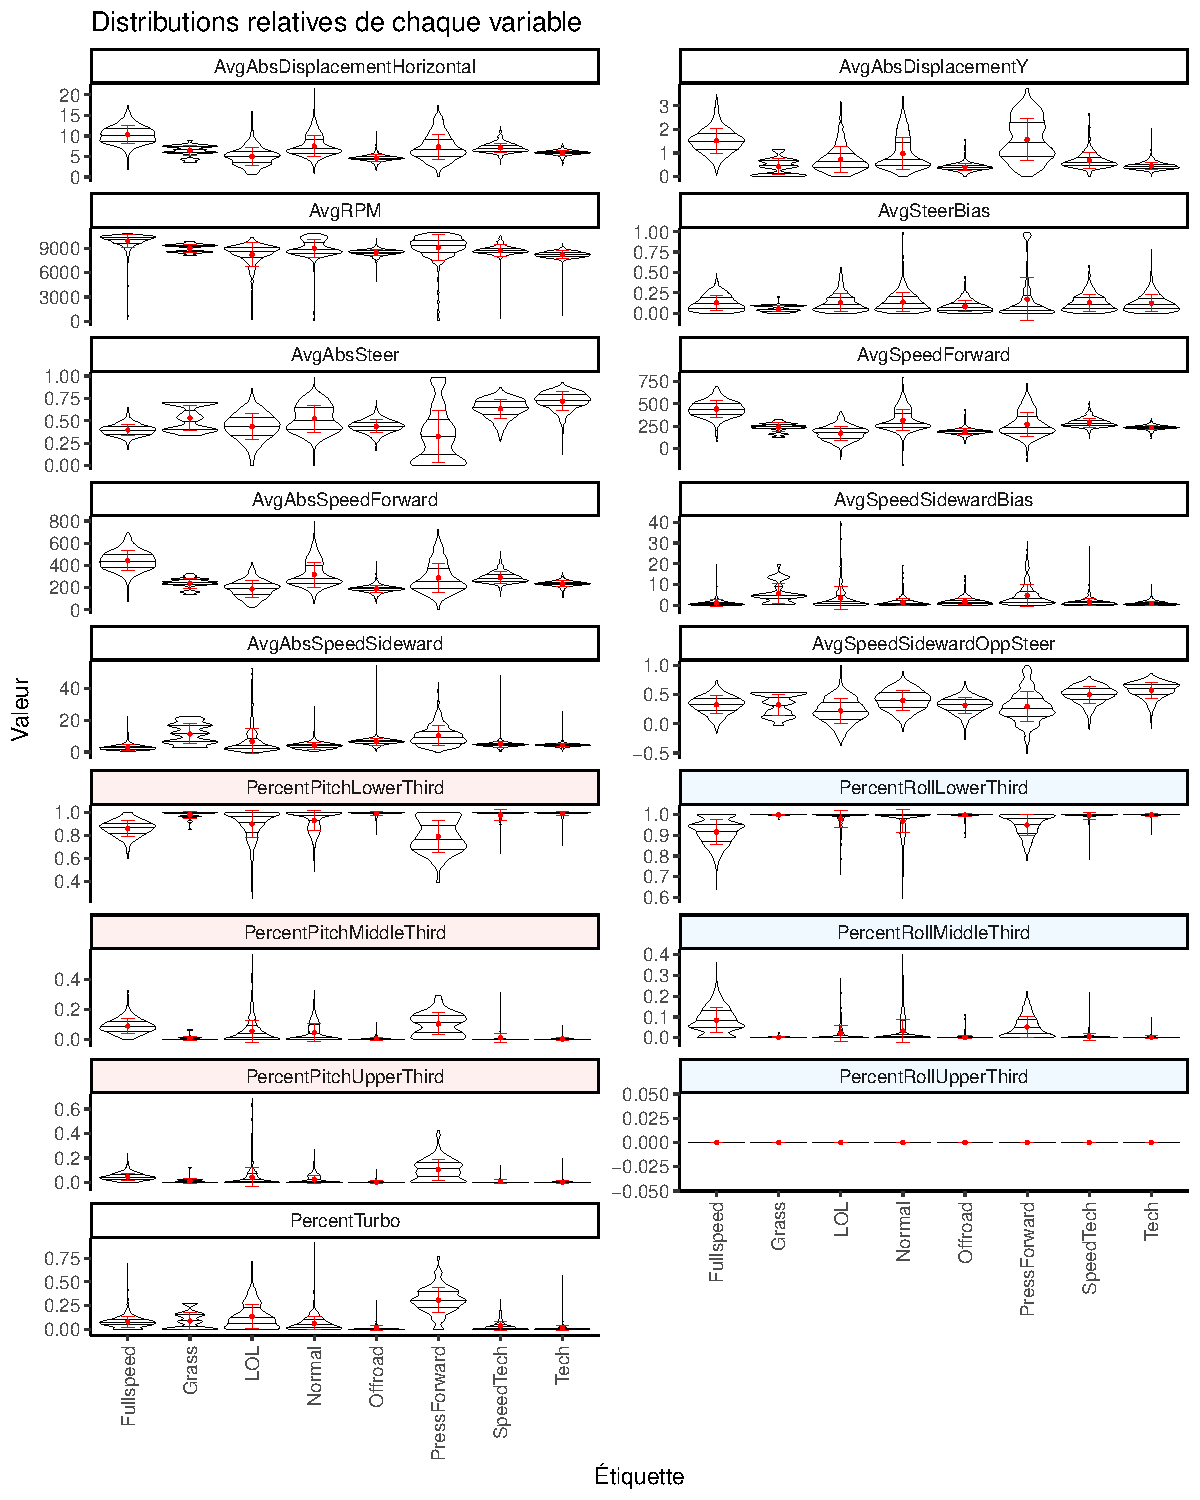
\includegraphics[width=1\textwidth,height=\textheight]{index_files/figure-pdf/fig-violin-facet-1.pdf}

}

\caption{\label{fig-violin-facet}Les distributions relatives (relatives
aux minimums et maximums) des valeurs de chaque variable selon
l'étiquette. Les barres rouges représentent l'écart type distancé de la
moyenne.}

\end{figure}%

\end{minipage}%

\end{figure}%

\subsection{Le variant}\label{le-variant}

Débutant avec des impressions générales, les circuits « PressForward »
ont les plus grandes variances. Ce motif suggère que cette étiquette
contient des circuits qui diffèrent grandement entre eux. Ceci est en
accord avec notre hypothèse originale selon laquelle la variance serait
présente dû à des acrobaties extrêmes. La présence d'acrobaties où la
voiture roulerait dans l'air est probablement ce qui a engendré les
variations des déplacements horizontaux
(\texttt{AvgAbsDisplacementHorizontal}) et verticaux
(\texttt{AvgAbsDisplacementY}), des vitesses vers l'avant
(\texttt{AvgSpeedForward}) et latérale (\texttt{AvgAbsSpeedSideward}),
et de l'orientation moyenne de la voiture (\texttt{PercentPitch——Third}
et \texttt{PercentRoll——Third}), démontrées dans la Figure
Figure~\ref{fig-violin-facet}.

Il est également notable que les circuits « PressForward » aient des
biais de pilotage (\texttt{AvgSteerBias}) et des pilotages totaux
(\texttt{AvgAbsSteer}) qui varient largement. Il y a plusieurs raisons
possibles. Si les circuits de cette étiquette suivent exactement le nom
--- seulement appuyer la touche avant ---, il n'y aurait aucun biais et
aucun pilotage. Ceci n'est pas le cas, mais il y a également la
possibilité qu'une touche directionnelle soit tenue le long du circuit.
Dans ce cas, le biais et le pilotage seraient chacun soit 0\% ou 100\%.
Ceci n'est également pas toujours le cas: les variables sont distribuées
d'une manière non binaire. Il y a ainsi des joueurs qui modifient leurs
entrées lors de leur cheminement. Il est donc plus difficile de
déterminer un motif pouvant identifier un circuit « PressForward » au
moyen d'un cheminement.

\subsection{L'impossibilité}\label{limpossibilituxe9}

La seule variable sans variance est le pourcentage de roulis se situant
dans le tiers le plus haut (\texttt{PercentRollUpperThird}). Bien que
ceci paraisse être en raison d'un manque de cheminements aberrants
plaçant la voiture à l'envers, ce n'est pas le cas. Plutôt, le calcul
qui convertit le quaternion de rotation vers le tangage, lacet et roulis
priorise le tangage au roulis. Il est ainsi impossible d'avoir un
pourcentage élevé de roulis dans le tiers maximal.

\subsection{Fullspeed}\label{fullspeed}

Les circuits « Fullspeed » ont, en moyenne, les plus grands déplacements
horizontaux (\texttt{AvgAbsDisplacementHorizontal}), révolutions par
minute (\texttt{AvgRPM}), vitesses vers l'avant
(\texttt{AvgSpeedForward}) et vitesses absolues vers l'avant
(\texttt{AvgAbsSpeedForward}), et sont plus souvent placés dans la zone
de roulis parallèle aux murs (\texttt{PercentRollMiddleThird}). Ceci
supporte nos hypothèses au sujet de l'étiquette « Fullspeed » et la
définition dès l'installation du jeu de 2020\footnote{Traduit, « Plein
  accélérateur le long du circuit. Longs virages fluides. Les boucles,
  la conduite sur les murs, et similaire sont communes. {[}\ldots{]} De
  hautes vitesses sont attendues. » (Eyebo {[}Rollins{]} 2024)}. L'appui
constant sur l'accélérateur élèverait les révolutions par minute du
moteur et la vitesse vers l'avant (\texttt{AvgSpeedForward} et
\texttt{AvgAbsSpeedForward}). Ajoutés à de hautes vitesses, des virages
prolongés pousseront la voiture à traverser une plus grande distance
(\texttt{AvgAbsDisplacementHorizontal}) durant son cheminement. Les
balades murales pourraient, ensuite, être la cause du haussement de
temps dans la zone de roulis situant la voiture près de perpendiculaire
au sol (\texttt{PercentRollMiddleThird}), soit parallèle aux murs.

\subsection{Circuits techniques}\label{circuits-techniques}

Nous avons posé l'hypothèse que les circuits ayant les étiquettes « Tech
» et « SpeedTech » se distingueraient par des pilotages et vitesses
pointant souvent dans des sens inverses. Ceci est, en effet, le cas,
visible dans la variable \texttt{AvgSpeedSidewardOppSteer}; les deux
étiquettes ont des moyennes de moyennes\footnote{C'est la moyenne de
  moyennes.} de vitesse latérale opposant le pilotage plus élevées
comparées aux autres étiquettes.

Plus intrigant encore, et que nous n'avons pas eu comme hypothèse: ces
deux étiquettes ont des distributions similaires, se différenciant de
manière prévisible. La « SpeedTech » réside à des vitesses
(\texttt{AvgSpeedForward} et \texttt{AvgAbsSpeedForward}), RPMs
(\texttt{AvgRPM}), durées en turbo (\texttt{PercentTurbo}) et
déplacements (\texttt{AvgAbsDisplacementHorizontal} et
\texttt{AvgAbsDisplacementY}) moyens légèrement plus hauts que les
circuits « Tech », comme ce que suggère l'utilisation du mot « Speed ».
Le « Tech », quant à lui, a plus de pilotage (\texttt{AvgAbsSteer}).
Notez que, dans le jeu, faire des virages serrés, ou même déraper,
ralenti la vitesse de la voiture. Les physiques du jeu soutiennent donc
que l'augmentation de montant de pilotage du « Tech » réduit sa vitesse
préférée, et inversement pour le « SpeedTech ». Les deux styles se
basant sur la technique sont donc fortement similaires, se différenciant
principalement par leurs caractéristiques de vitesse préférée.

\subsection{Le grass-slide}\label{le-grass-slide}

D'abord, nous avons eu l'hypothèse que l'étiquette « Grass » se
distinguerait par une hausse de vitesse angulaire et de vitesse
latérale. Les distributions de la variable \texttt{AvgAbsSpeedSideward},
ou la vitesse latérale absolue moyenne, supportent ceci. La moyenne de
celui-ci pour les circuits « Grass » est la plus élevée parmi les autres
étiquettes.

\section{Quel modèle de classification est le plus représentatif
?}\label{quel-moduxe8le-de-classification-est-le-plus-repruxe9sentatif}

Nous avons décidé d'utiliser un modèle d'amplification de gradients à
classes multiples comme modèle principal, tel que décrit dans la section
« Quel modèle de classification servira le mieux ? ». Les paramètres de
ce modèle ont été raffinés afin de l'optimiser. En premier lieu, la
profondeur maximale de l'arbre est de cinq afin de prévenir le
surajustement du modèle aux données d'entraînement. La mesure
d'évaluation que le modèle cherche à optimiser est la perte logistique
multiclasse, ayant comme calcul, pour chaque variable individuellement,

\(\[L_{log}(y,p) = -(y\log{p} + (1 - y)\log{1 - p})\]\)

\section{Que peut être déduit au sujet des affectants de l'étiquette
résultante grâce aux modèles
?}\label{que-peut-uxeatre-duxe9duit-au-sujet-des-affectants-de-luxe9tiquette-ruxe9sultante-gruxe2ce-aux-moduxe8les-1}

\chapter{Résultats}\label{sec-result}

\begin{figure}[H]

\centering{

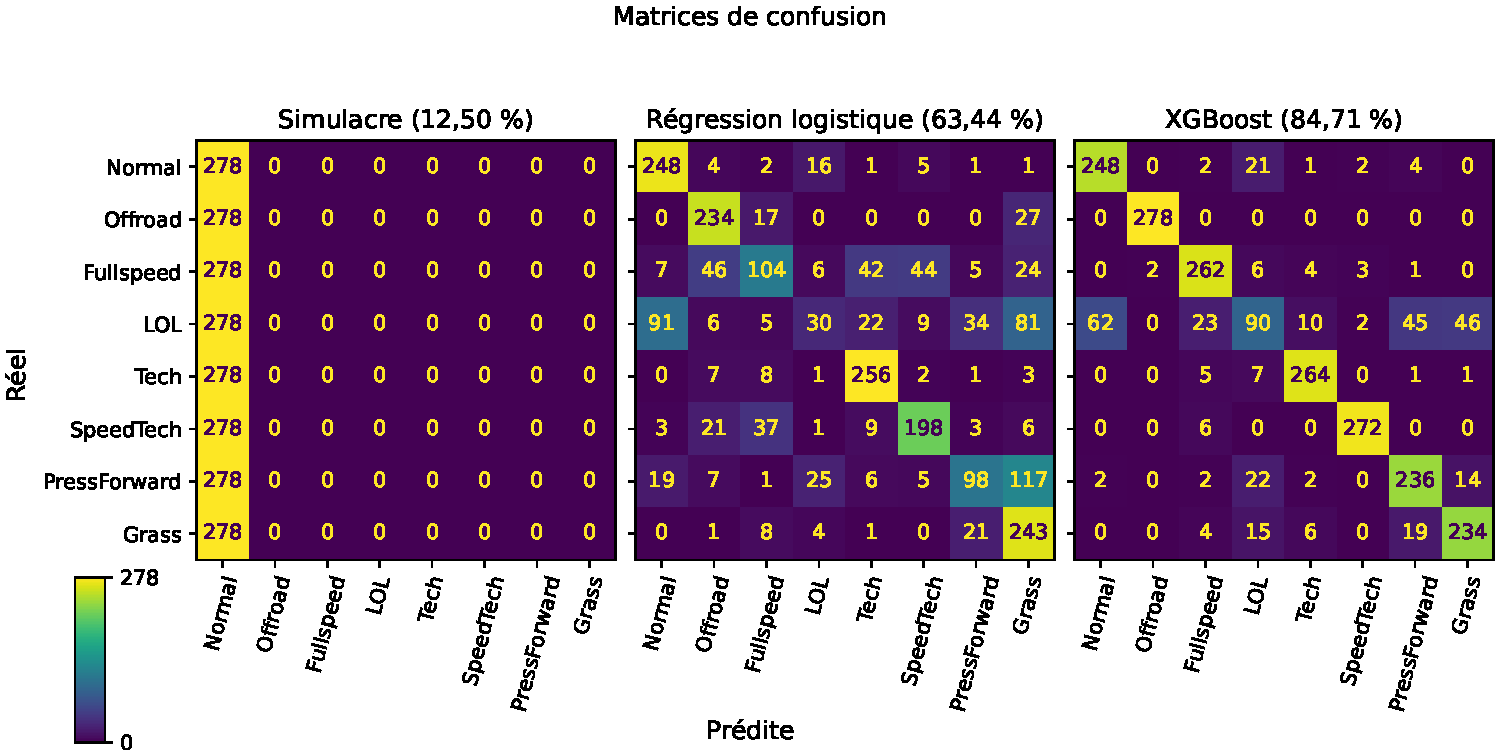
\includegraphics{rendered-figs/fig-model-stats.pdf}

}

\caption{\label{fig-model-stats}Les matrices de confusion des trois
modèles statistiques utilisés: un simulacre simple, une régression
logistique, et un amplification de gradients (XGBoost).}

\end{figure}%

\begin{longtable}[t]{lllllll}

\toprule
\multicolumn{1}{c}{ } & \multicolumn{2}{c}{Simulacre} & \multicolumn{2}{c}{\makecell[c]{Régression\\logistique}} & \multicolumn{2}{c}{\makecell[c]{Amplification\\de gradients}} \\
\cmidrule(l{3pt}r{3pt}){2-3} \cmidrule(l{3pt}r{3pt}){4-5} \cmidrule(l{3pt}r{3pt}){6-7}
Étiquette & Précision & Rappel & Précision & Rappel & Précision & Rappel\\
\midrule
Normal & 12,50 & 100 & 67,39 & 89,21 & 79,49 & 89,21\\
Offroad & 0 & 0 & 71,78 & 84,17 & 99,29 & 100\\
Fullspeed & 0 & 0 & 57,14 & 37,41 & 86,18 & 94,24\\
LOL & 0 & 0 & 36,14 & 10,79 & 55,90 & 32,37\\
Tech & 0 & 0 & 75,96 & 92,09 & 91,99 & 94,96\\
\addlinespace
SpeedTech & 0 & 0 & 75,29 & 71,22 & 97,49 & 97,84\\
PressForward & 0 & 0 & 60,12 & 35,25 & 77,12 & 84,89\\
Grass & 0 & 0 & 48,41 & 87,41 & 79,32 & 84,17\\
\cellcolor[HTML]{e6e6e6}{\textbf{Moyenne}} & \cellcolor[HTML]{e6e6e6}{\textbf{1,56}} & \cellcolor[HTML]{e6e6e6}{\textbf{12,50}} & \cellcolor[HTML]{e6e6e6}{\textbf{61,53}} & \cellcolor[HTML]{e6e6e6}{\textbf{63,44}} & \cellcolor[HTML]{e6e6e6}{\textbf{83,35}} & \cellcolor[HTML]{e6e6e6}{\textbf{84,71}}\\
\bottomrule


\caption{\label{tbl-rapport-classification}La précision et le rappel de
chaque model selon la variable, en pourcentage (\%).}

\tabularnewline
\end{longtable}

\begin{figure}[H]

\centering{

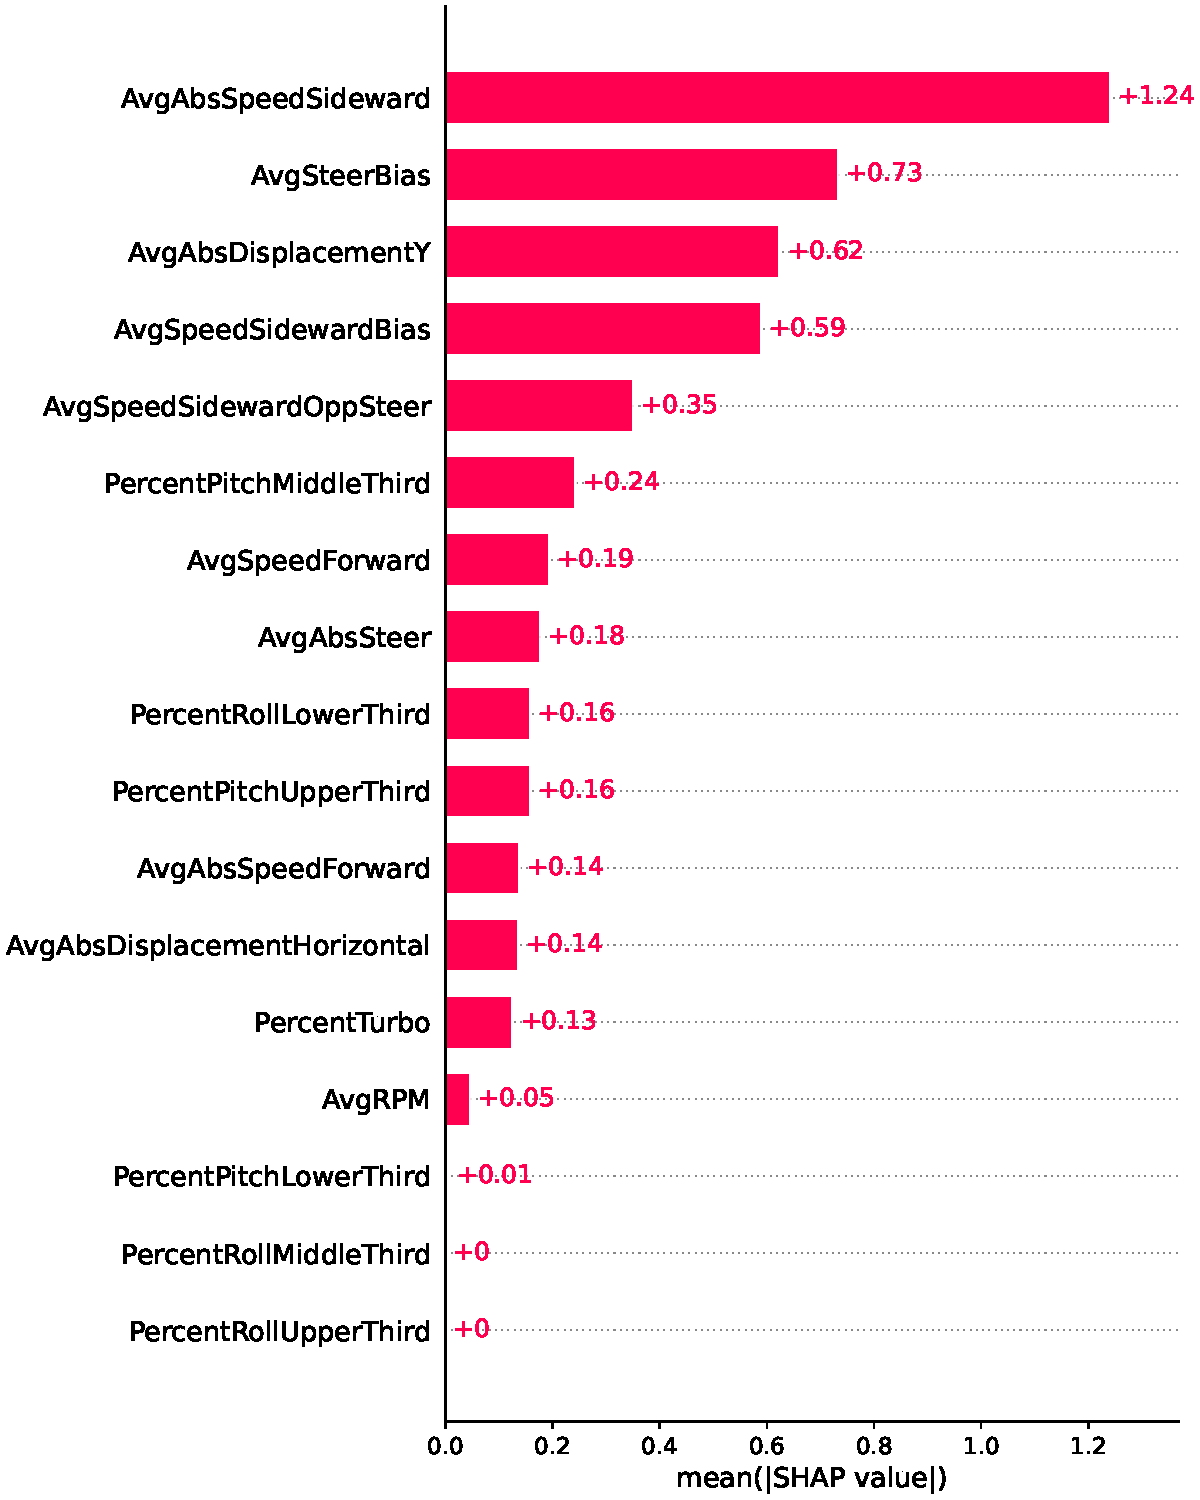
\includegraphics{rendered-figs/fig-bar.pdf}

}

\caption{\label{fig-importance-bar}La moyenne absolue des valeurs SHAP
de chaque variable indépendante.}

\end{figure}%

\begin{figure}[H]

\centering{

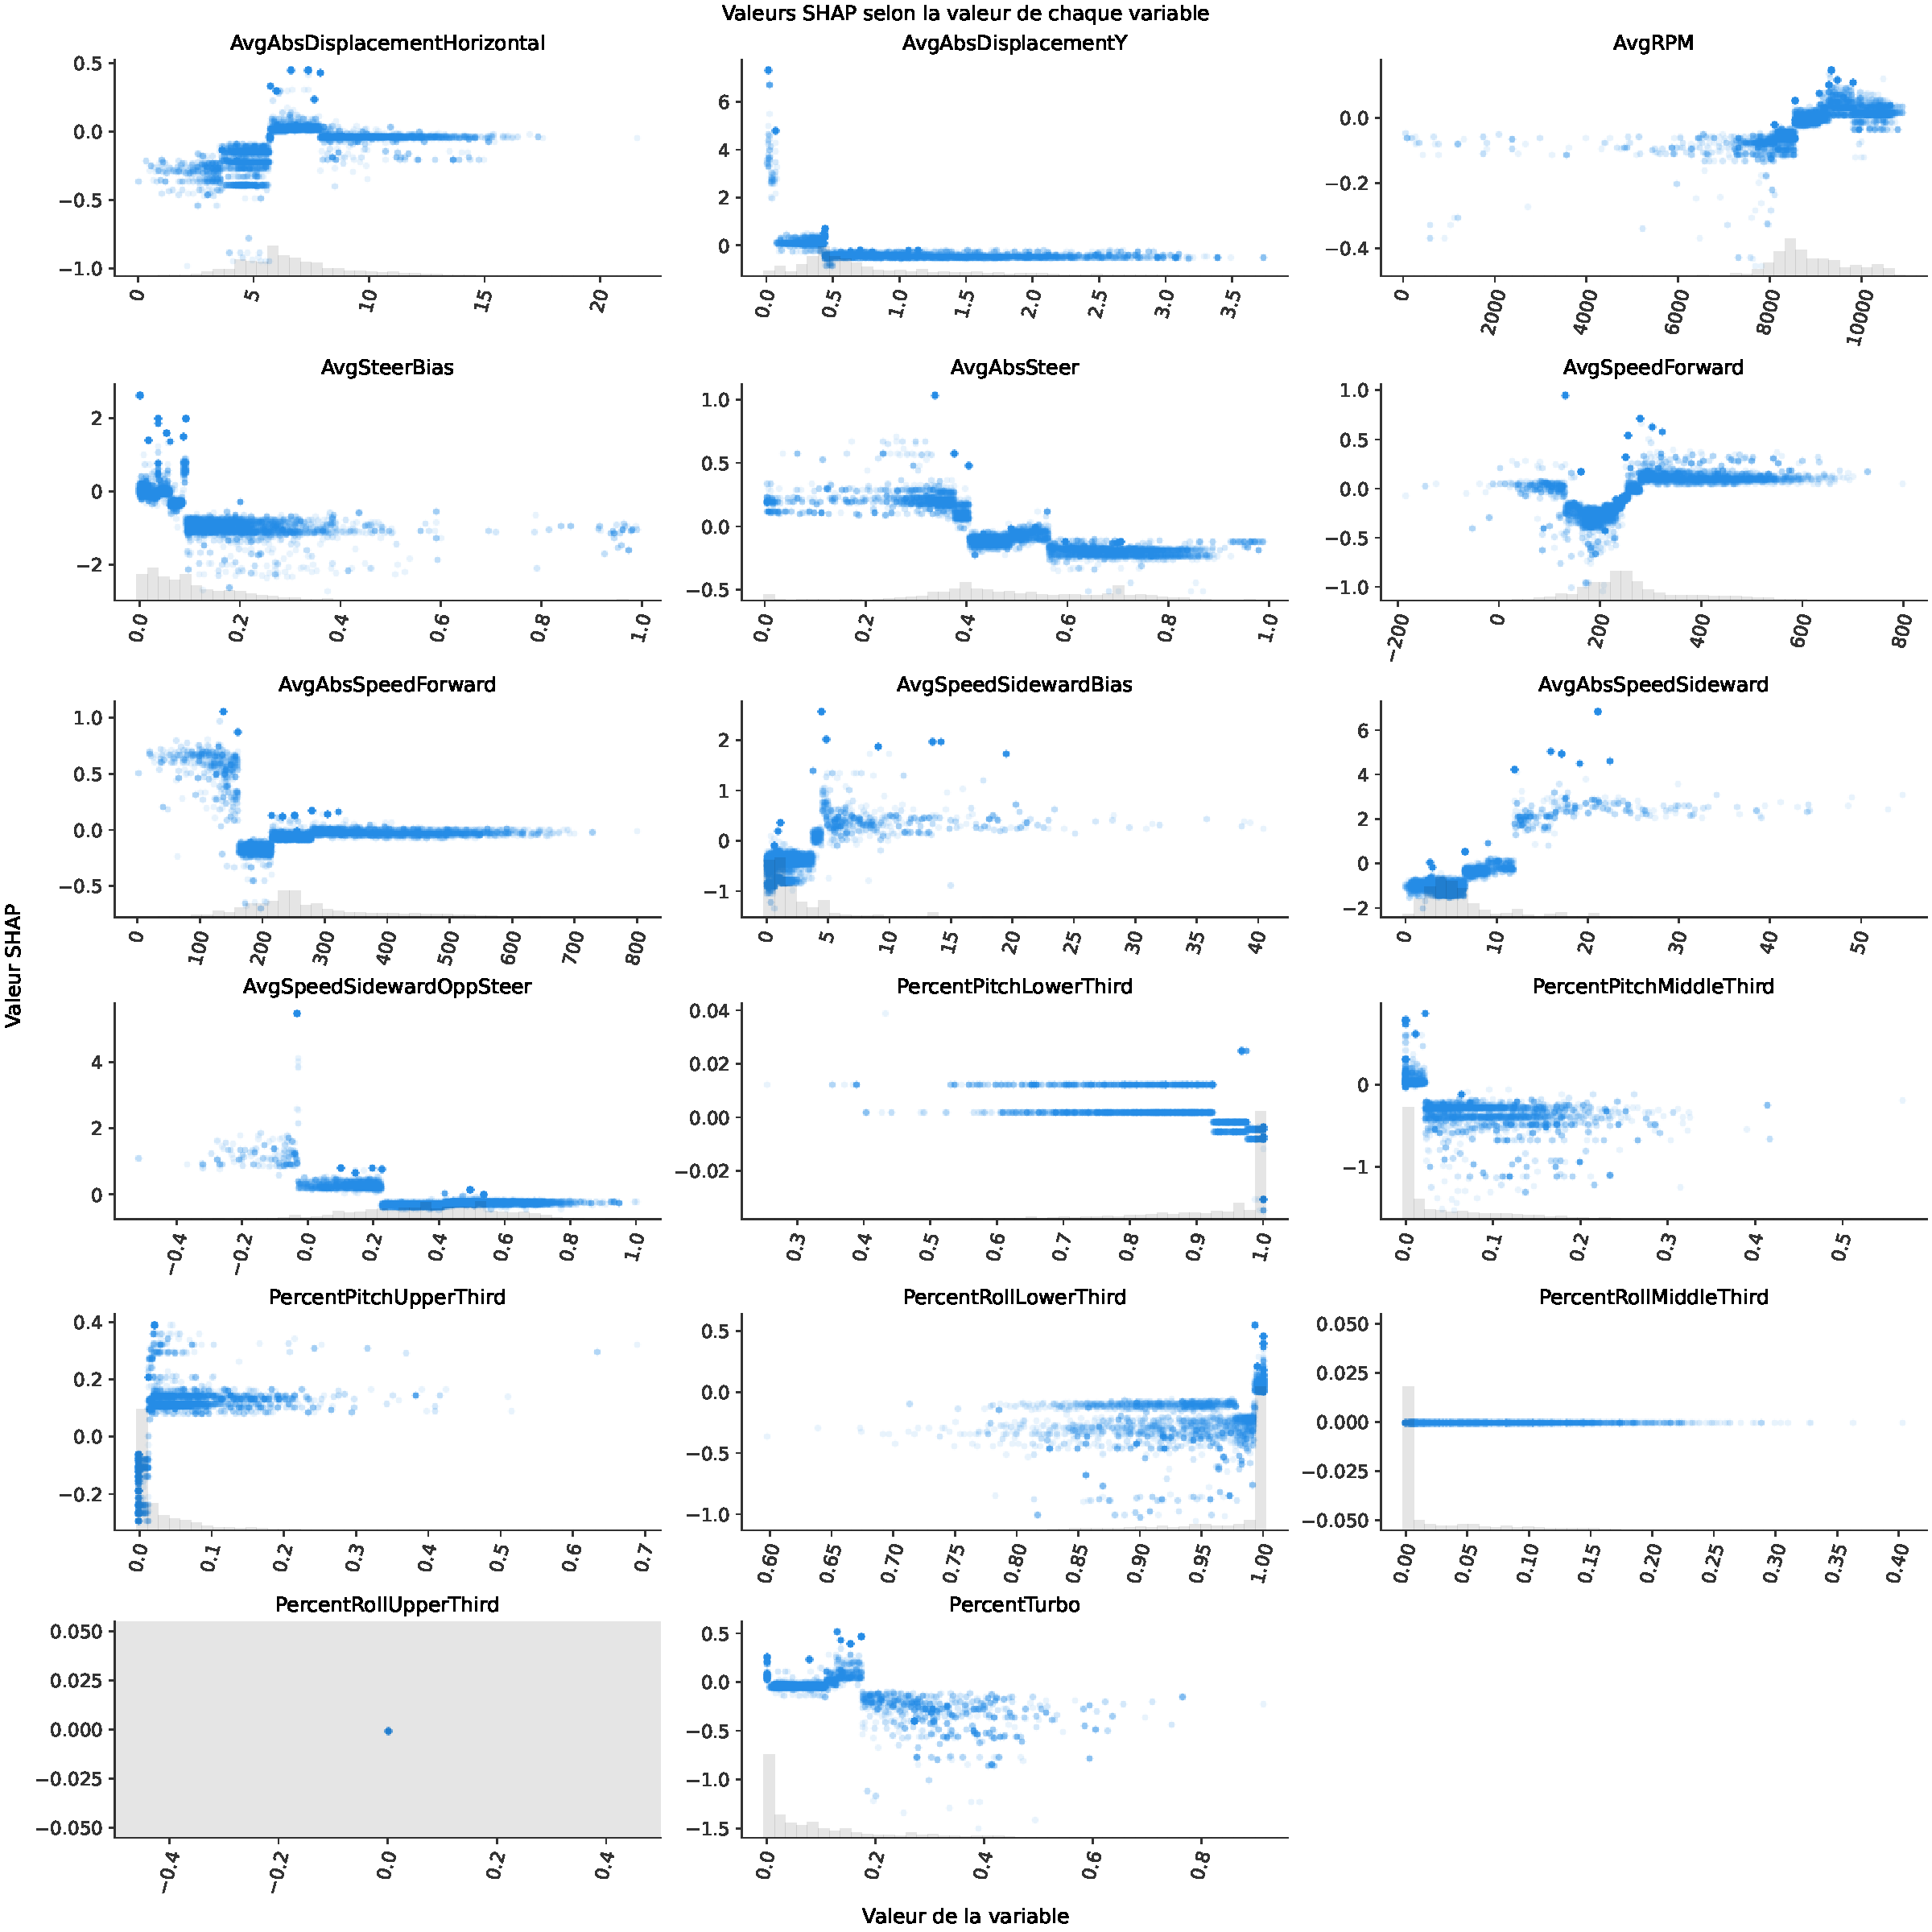
\includegraphics{rendered-figs/fig-scatter.pdf}

}

\caption{\label{fig-scatter}Les corrélations entre la valeur SHAP et la
valeur de chaque variable. Les barres grises indiquent la dansité.}

\end{figure}%

\begin{figure}[H]

\centering{

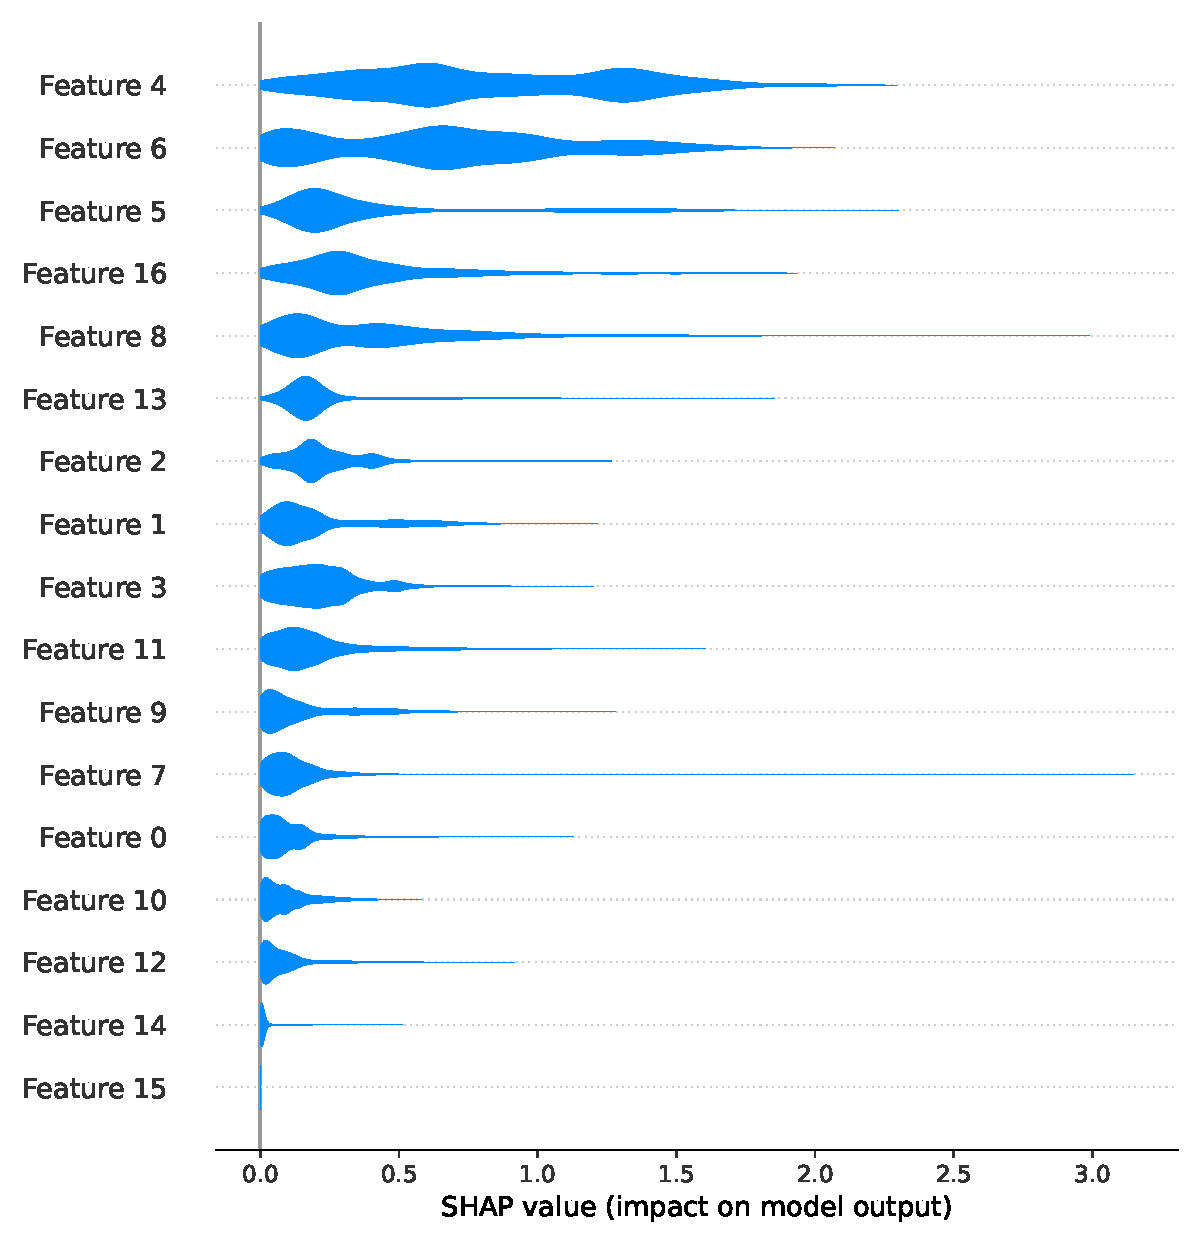
\includegraphics{rendered-figs/fig-violin.pdf}

}

\caption{\label{fig-violin}\ldots\ldots\ldots\ldots\ldots.}

\end{figure}%

\begin{figure}[H]

\centering{

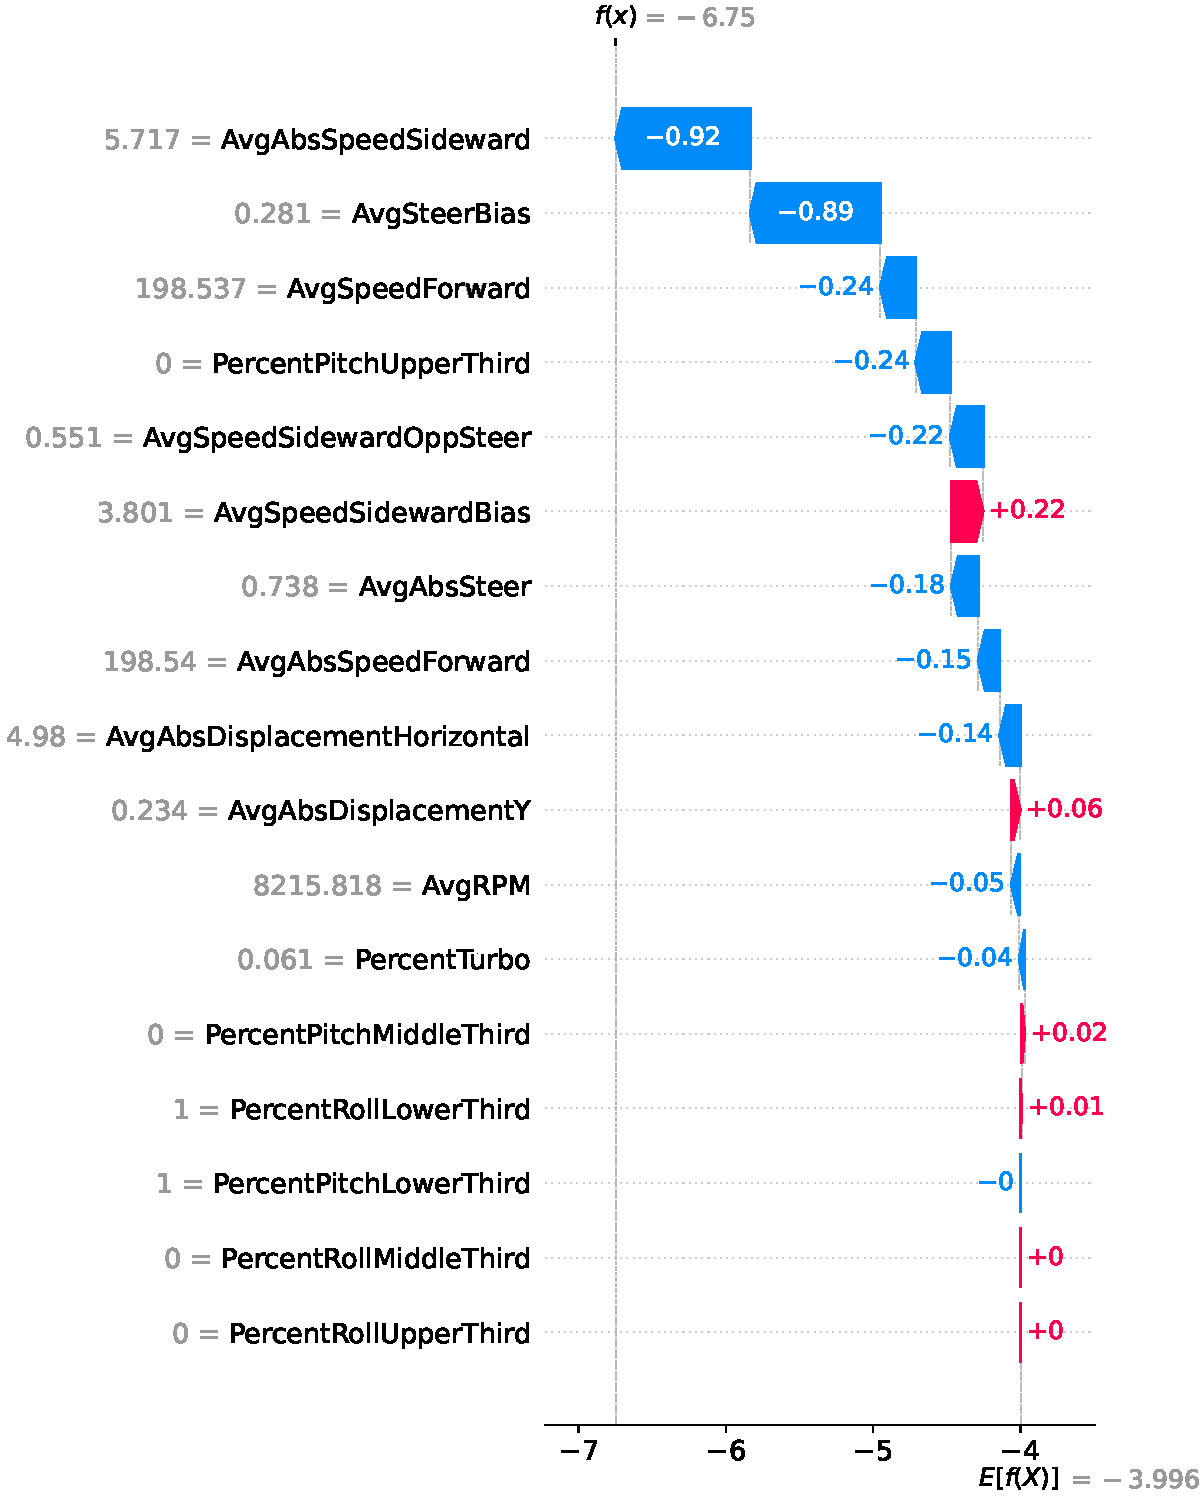
\includegraphics{rendered-figs/fig-waterfall-0.pdf}

}

\caption{\label{fig-waterfall-0}\ldots\ldots\ldots\ldots\ldots.}

\end{figure}%

\chapter{Discussion}\label{sec-discussion}

\chapter{Conclusion}\label{sec-conclusion}

\chapter{Bibliographie}\label{sec-bib}

\phantomsection\label{refs}
\begin{CSLReferences}{1}{0}
\bibitem[\citeproctext]{ref-base}

\bibitem[\citeproctext]{ref-rmarkdown}
Allaire, JJ, Yihui Xie, Christophe Dervieux, Jonathan McPherson, Javier
Luraschi, Kevin Ushey, Aron Atkins, et al. 2024. \emph{rmarkdown:
Dynamic Documents for R}. \url{https://github.com/rstudio/rmarkdown}.

\bibitem[\citeproctext]{ref-IntroXAI}
{«~An introduction to explainable AI with Shapley values~»}. 2018.
\emph{SHAP}.
\url{https://shap.readthedocs.io/en/latest/example_notebooks/overviews/An\%20introduction\%20to\%20explainable\%20AI\%20with\%20Shapley\%20values.html}.

\bibitem[\citeproctext]{ref-ArchimeaTMWiki}
Archimëa, et al. 2015. \emph{TrackMania}.
https://fr.wikipedia.org/wiki/TrackMania: Wikipédia.

\bibitem[\citeproctext]{ref-AwanIntroSHAP}
Awan, Abid Ali. 2015. \emph{An Introduction to SHAP Values and Machine
Learning Interpretability}.
https://www.datacamp.com/tutorial/introduction-to-shap-values-machine-learning-interpretability:
DataCamp.

\bibitem[\citeproctext]{ref-BertrandNewton}
Bertrand, Emile. 2024. \emph{Lois du mouvement de Newton}.
https://fr.wikipedia.org/wiki/Lois\_du\_mouvement\_de\_Newton:
Wikipédia.

\bibitem[\citeproctext]{ref-XGBoostingSampleMethod}
Brownlee, Jason. s.~d. {«~Configure XGBoost "sampling\_method"
Parameter~»}. \emph{XGBoosting}.
\url{https://xgboosting.com/configure-xgboost-sampling_method-parameter/}.

\bibitem[\citeproctext]{ref-ChawlaAIResearch}
Chawla, Nitesh V., et al. 2002. {«~SMOTE: Synthetic Minority
Over-sampling Technique~»}. \emph{Journal of Artificial Intelligence
Research}. https://doi.org/\url{https://doi.org/10.1613/jair.953}.

\bibitem[\citeproctext]{ref-XGBoostScalable}
Chen, Tianqi and Carlos Guestrin. 2016. {«~XGBoost: {A} Scalable Tree
Boosting System~»}. \emph{CoRR}.
https://doi.org/\url{https://doi.org/10.48550/arXiv.1603.02754}.

\bibitem[\citeproctext]{ref-ggbeeswarm}
Clarke, Erik, Scott Sherrill-Mix, et Charlotte Dawson. 2023.
\emph{ggbeeswarm: Categorical Scatter (Violin Point) Plots}.
\url{https://github.com/eclarke/ggbeeswarm}.

\bibitem[\citeproctext]{ref-rjson}
Couture-Beil, Alex. 2024. \emph{rjson: JSON for R}.
\url{https://github.com/alexcb/rjson}.

\bibitem[\citeproctext]{ref-WaryCausalInsights}
Dillon, Eleanor, et al. 2018. {«~Be careful when interpreting predictive
models in search of causal insights~»}. \emph{SHAP}.
\url{https://shap.readthedocs.io/en/latest/example_notebooks/overviews/Be\%20careful\%20when\%20interpreting\%20predictive\%20models\%20in\%20search\%20of\%20causal\%20insights.html}.

\bibitem[\citeproctext]{ref-Eyebo2024}
Eyebo {[}Rollins{]}. 2024. {«~Tags Explained~»}. \emph{Trackmania 2020
Exchange}. \url{https://trackmania.exchange/threads/700/tags-explained}.

\bibitem[\citeproctext]{ref-ResearchApproaches}
Faculty of Environment. s.~d. {«~Types of research approaches~»}.
\emph{University of Waterloo School of Planning}.
\url{https://uwaterloo.ca/planning/current-undergraduate-students/student-program-page/senior-courses-interest/types-research-approaches}.

\bibitem[\citeproctext]{ref-janitor}
Firke, Sam. 2023. \emph{janitor: Simple Tools for Examining and Cleaning
Dirty Data}. \url{https://github.com/sfirke/janitor}.

\bibitem[\citeproctext]{ref-viridis}
Garnier, Simon. 2024. \emph{viridis: Colorblind-Friendly Color Maps for
R}. \url{https://sjmgarnier.github.io/viridis/}.

\bibitem[\citeproctext]{ref-viridis2024}
Garnier, Simon, Ross, Noam, Rudis, Robert, Camargo, et al. 2024.
\emph{{viridis(Lite)} - Colorblind-Friendly Color Maps for R}.
\url{https://doi.org/10.5281/zenodo.4679423}.

\bibitem[\citeproctext]{ref-XGBoostStart}
{«~Getting started with XGBoost~»}. 2022. \emph{XGBoost Python Package}.
\url{https://xgboost.readthedocs.io/en/stable/python/examples/basic_walkthrough.html\#sphx-glr-python-examples-basic-walkthrough-py}.

\bibitem[\citeproctext]{ref-GuptaPrecisionRecall}
Gupta, Mehul. 2020. {«~Calculating Precision \& Recall for Multi-Class
Classification~»}. \emph{Medium}.
\url{https://medium.com/data-science-in-your-pocket/calculating-precision-recall-for-multi-class-classification-9055931ee229}.

\bibitem[\citeproctext]{ref-TrialIbazz}
iBazztyB, et al. s.~d. {«~Maps~»}. \emph{Trackmania Trial Website}.
\url{https://www.tmrpgtrial.com/maps}.

\bibitem[\citeproctext]{ref-SVM2019}
Iranmehr, Arya, et al. 2019. {«~Cost-sensitive support vector
machines~»}. \emph{Neurocomputing}.
https://doi.org/\url{https://doi.org/10.1016/j.neucom.2018.11.099}.

\bibitem[\citeproctext]{ref-JstAnothr}
JstAnothrVirtuoso. 2024. {«~The WR Race - TMUF!~»} \emph{Youtube}.
\url{https://www.youtube.com/watch?v=zn0h9mrIgpU}.

\bibitem[\citeproctext]{ref-KattackMultiLabel}
Kattack, et al. 2006. {«~Multi-label classification~»}.
\emph{Wikipedia}.
\url{https://en.wikipedia.org/wiki/Multi-label_classification}.

\bibitem[\citeproctext]{ref-KeitaIntroClassification}
Keita, Zoumana. 2024. {«~Classification in Machine Learning: An
Introduction~»}. \emph{Datacamp}.
\url{https://www.datacamp.com/blog/classification-machine-learning}.

\bibitem[\citeproctext]{ref-EO2EnduranceTAS}
Kimura, et al. 2021. {«~{[}Trackmania TAS{]} E02-Endurance 1:31.52
(-1:55.06) ft.Niro \& Shweetz~»}. \emph{YouTube}.
\url{https://www.youtube.com/watch?v=GpDu8ITfSSE}.

\bibitem[\citeproctext]{ref-EasyPF}
Kmita, Nicolas. 2022. {«~Easy Press-Forward~»}. \emph{TMNF-X}.
\url{https://tmnf.exchange/trackshow/9797488}.

\bibitem[\citeproctext]{ref-GBXPos}
---------. s.~d. {«~GBXPosBlenderAddon~»}. \emph{Github}.
\url{https://github.com/DarkMattrMaestro/GBXPosBlenderAddon}.

\bibitem[\citeproctext]{ref-academie}
L'académie française. 2019. {«~Dictionnaire de l'Académie française~»}.
\url{https://www.dictionnaire-academie.fr/}.

\bibitem[\citeproctext]{ref-scikitLogLoss}
{«~log\_loss~»}. 2024. \emph{scikit-learn 1.6.0 documentation}.
\url{https://scikit-learn.org/stable/modules/generated/sklearn.metrics.log_loss.html}.

\bibitem[\citeproctext]{ref-TMNFX}
Mania.Exchange. s.~d. {«~TMNF-X~»}. \url{https://tmnf.exchange/}.

\bibitem[\citeproctext]{ref-PatrickQuartoTips}
Patrick, Cameron. 2023. {«~Some Quarto PDF formatting tips, with
particular reference to thesis writing~»}. \emph{Posting completely at
random}.
\url{https://cameronpatrick.com/post/2023/07/quarto-thesis-formatting/}.

\bibitem[\citeproctext]{ref-Linesight}
pb4git, et al. 2024. {«~I Trained an AI for 2 Years on Trackmania. It's
Breaking Records~»}. \emph{YouTube}.
\url{https://www.youtube.com/watch?v=cUojVsCJ51I}.

\bibitem[\citeproctext]{ref-BigBang1112}
Pivoňka, Petr. s.~d.a. {«~BigBang1112 (Petr Pivoňka)~»}. \emph{GitHub}.
\url{https://github.com/BigBang1112}.

\bibitem[\citeproctext]{ref-GBXNetExplorer}
---------. s.~d.b. {«~GBX.Net Explorer~»}. \emph{GBX Tools}.
\url{https://explorer.gbx.tools/}.

\bibitem[\citeproctext]{ref-GBXNET}
Pivoňka, Petr, et al. s.~d. {«~GBX.NET~»}. \emph{Github}.
\url{https://github.com/BigBang1112/gbx-net}.

\bibitem[\citeproctext]{ref-PoldrackStatModeling}
Poldrack, Russell A. 2021. {«~30.1: The Process of Statistical
Modeling~»}. \emph{Statistics LibreTexts}.
\url{https://stats.libretexts.org/Bookshelves/Introductory_Statistics/Statistical_Thinking_for_the_21st_Century_(Poldrack)/30\%3A_Practical_statistical_modeling/30.01\%3A_The_Process_of_Statistical_Modeling}.

\bibitem[\citeproctext]{ref-DMatrix}
{«~Python API Reference - DMatrix~»}. 2022. \emph{XGBoost Python
Package}.
\url{https://xgboost.readthedocs.io/en/stable/python/python_api.html\#xgboost.DMatrix}.

\bibitem[\citeproctext]{ref-Allure}
{«~Résultats - allure~»}. s.~d. \emph{Base de données lexicographiques
panfrancophone}. \url{https://www.bdlp.org/resultat?&query=allure~}.

\bibitem[\citeproctext]{ref-HypertuningXGBoost}
RITHP. 2023. {«~Optimizing XGBoost: A Guide to Hyperparameter Tuning~»}.
\emph{Medium}.
\url{https://medium.com/@rithpansanga/optimizing-xgboost-a-guide-to-hyperparameter-tuning-77b6e48e289d}.

\bibitem[\citeproctext]{ref-scikitPrecisionRecall}
scikit-learn developers. 2024. {«~Precision-Recall~»}.
\emph{scikit-learn 1.6.0 documentation}.
\url{https://scikit-learn.org/stable/auto_examples/model_selection/plot_precision_recall.html}.

\bibitem[\citeproctext]{ref-TMNFXStats}
{«~Site Statistics~»}. s.~d. \emph{Trackmania Nations Forever Exchange}.
\url{https://tmnf.exchange/statistics}.

\bibitem[\citeproctext]{ref-wikiPrincipalAxes}
Skyerise, et al. 2007. {«~Aircraft principal axes~»}. \emph{Wikipedia}.
\url{https://en.wikipedia.org/wiki/Aircraft_principal_axes}.

\bibitem[\citeproctext]{ref-FoolingLIMEandSHAP}
Slack, Dylan, et al. 2019. {«~Fooling LIME and SHAP: Adversarial Attacks
on Post hoc Explanation Methods~»}. \emph{CoRR}.
https://doi.org/\url{https://doi.org/10.48550/arXiv.1911.02508}.

\bibitem[\citeproctext]{ref-TMDojo}
TeamDojo. s.~d. {«~TMDojo~»}. \url{https://tmdojo.com/}.

\bibitem[\citeproctext]{ref-QuatToPYR}
thewhiteambit. 2019. {«~python 3.x - Quaternion to Yaw pitch roll~»}.
\emph{Stack Overflow}.
\url{https://stackoverflow.com/questions/54214698/quaternion-to-yaw-pitch-roll}.

\bibitem[\citeproctext]{ref-TomekUnlimiter}
Tomek0055. 2016. {«~TrackMania Unlimiter 2.0 (ver: 31.05.2024)~»}.
\emph{TMUF-X}.
\url{https://tmuf.exchange/threadshow/4724293?&postId=4724294}.

\bibitem[\citeproctext]{ref-TrevisanSHAP}
Trevisan, Vinícius. 2022. {«~Using SHAP Values to Explain How Your
Machine Learning Model Works~»}. \emph{Medium}.
\url{https://towardsdatascience.com/using-shap-values-to-explain-how-your-machine-learning-model-works-732b3f40e137}.

\bibitem[\citeproctext]{ref-Tunachopps}
Tunachopps. 2023. {«~Best way to get better at bugslides?~»}
\emph{Reddit}.
\url{https://www.reddit.com/r/TrackMania/comments/13iwa0y/comment/jkccn9o/}.

\bibitem[\citeproctext]{ref-XGBoostPythonDatacamp}
Tuychiev, Bekhruz. 2023. {«~Using XGBoost in Python Tutorial~»}.
\emph{Datacamp}.
\url{https://www.datacamp.com/tutorial/xgboost-in-python}.

\bibitem[\citeproctext]{ref-reticulate}
Ushey, Kevin, JJ Allaire, et Yuan Tang. 2024. \emph{reticulate:
Interface to 'Python'}. \url{https://rstudio.github.io/reticulate/}.

\bibitem[\citeproctext]{ref-ggh4x}
van den Brand, Teun. 2024. \emph{ggh4x: Hacks for 'ggplot2'}.
\url{https://github.com/teunbrand/ggh4x}.

\bibitem[\citeproctext]{ref-FloatingPoint}
Wagner, Bill, et al. 2022. {«~Floating-point numeric types - C\#
reference~»}. \emph{Microsoft Learn}.
\url{https://learn.microsoft.com/en-us/dotnet/csharp/language-reference/builtin-types/floating-point-numeric-types}.

\bibitem[\citeproctext]{ref-HuggingTabular2022}
{«~What is Tabular Classification?~»} 2022. \emph{Hugging Face}.
\url{https://huggingface.co/tasks/tabular-classification}.

\bibitem[\citeproctext]{ref-reshape2007}
Wickham, Hadley. 2007. {«~Reshaping data with the reshape package~»}.
\emph{Journal of Statistical Software} 21 (12).
\url{https://www.jstatsoft.org/v21/i12/}.

\bibitem[\citeproctext]{ref-reshape}
---------. 2022. \emph{reshape: Flexibly Reshape Data}.
\url{http://had.co.nz/reshape}.

\bibitem[\citeproctext]{ref-tidyverse}
---------. 2023. \emph{tidyverse: Easily Install and Load the
'Tidyverse'}. \url{https://tidyverse.tidyverse.org}.

\bibitem[\citeproctext]{ref-tidyverse2019}
Wickham, Hadley, Mara Averick, Jennifer Bryan, Winston Chang, Lucy
D'Agostino McGowan, Romain François, Garrett Grolemund, et al. 2019.
{«~Welcome to the {tidyverse}~»}. \emph{Journal of Open Source Software}
4 (43): 1686. \url{https://doi.org/10.21105/joss.01686}.

\bibitem[\citeproctext]{ref-XGBoostMultiOutput}
XGBoost. 2022. {«~Multiple Outputs~»}. \emph{XGBoost 2.1.1
Documentation}.
\url{https://xgboost.readthedocs.io/en/stable/tutorials/multioutput.html}.

\bibitem[\citeproctext]{ref-knitr2014}
Xie, Yihui. 2014. {«~knitr: A Comprehensive Tool for Reproducible
Research in {R}~»}. In \emph{Implementing Reproducible Computational
Research}, édité par Victoria Stodden, Friedrich Leisch, et Roger D.
Peng. Chapman; Hall/CRC.

\bibitem[\citeproctext]{ref-knitr2015}
---------. 2015. \emph{Dynamic Documents with {R} and knitr}. 2nd éd.
Boca Raton, Florida: Chapman; Hall/CRC. \url{https://yihui.org/knitr/}.

\bibitem[\citeproctext]{ref-tinytex2019}
---------. 2019. {«~TinyTeX: A lightweight, cross-platform, and
easy-to-maintain LaTeX distribution based on TeX Live~»}. \emph{TUGboat}
40 (1): 30‑32. \url{https://tug.org/TUGboat/Contents/contents40-1.html}.

\bibitem[\citeproctext]{ref-knitr}
---------. 2024a. \emph{knitr: A General-Purpose Package for Dynamic
Report Generation in R}. \url{https://yihui.org/knitr/}.

\bibitem[\citeproctext]{ref-tinytex}
---------. 2024b. \emph{tinytex: Helper Functions to Install and
Maintain TeX Live, and Compile LaTeX Documents}.
\url{https://github.com/rstudio/tinytex}.

\bibitem[\citeproctext]{ref-rmarkdown2018}
Xie, Yihui, J. J. Allaire, et Garrett Grolemund. 2018. \emph{R Markdown:
The Definitive Guide}. Boca Raton, Florida: Chapman; Hall/CRC.
\url{https://bookdown.org/yihui/rmarkdown}.

\bibitem[\citeproctext]{ref-rmarkdown2020}
Xie, Yihui, Christophe Dervieux, et Emily Riederer. 2020. \emph{R
Markdown Cookbook}. Boca Raton, Florida: Chapman; Hall/CRC.
\url{https://bookdown.org/yihui/rmarkdown-cookbook}.

\bibitem[\citeproctext]{ref-Yosh}
{«~Yosh~»}. s.~d. \emph{YouTube}. \url{https://www.youtube.com/@yoshtm}.

\bibitem[\citeproctext]{ref-kableExtra}
Zhu, Hao. 2024. \emph{kableExtra: Construct Complex Table with 'kable'
and Pipe Syntax}. \url{http://haozhu233.github.io/kableExtra/}.

\end{CSLReferences}

\chapter{Annexe}\label{sec-annex}




\end{document}
